\documentclass[12pt,fleqn]{article}\usepackage{../common}
\begin{document}
Ders 9

Sabit Katsayili (Coefficients) Lineer 2. Seviye ODE'ler 

Standart formu su sekildedir

\[ y'' + Ay' + By = 0 \]

Sifira esit olmasi denklemin homojen oldugu anlamina gelir. $A$ ve $B$
sabittir. Bu denklemin en genel hali degildir, mesela $A$ ya da $B$
bagimsiz degiskenin ($x$, $t$, vs) bir fonksiyonu ise daha genel
olabilir. Sag kisim 0 yerine bir fonksiyon ise o zaman denklem homojen
olmayan (inhomogeneous) demektir. O tur denklemlerin fiziksel baglamda ayri
bir anlami var tabii, o yuzden once homojen denklemler incelenmeye
baslanir, sonra homojenlige olmayan duruma gecilir.

Genel cozumun soyle oldugunu farz edelim

\[ y = c_1 y_1 + c_2 y_2 \]

Cozumde iki tane rasgele (arbitrary) sabit olmasinin sezgisel bir tarifi
sudur: Denklem 2. derece, ve $y''$'den $y$'yi elde etmek icin iki kere
entegre etmek gereklidir, ve o sirada entegrasyon sonucu sonuca ardi ardina
iki tane rasgele sabit ekler, kabaca bir tarif boyledir. Niye ayri $y_1$ ve
$y_2$?  Mesela $c_1 = 0, c_2 = 1$ diyelim, o zaman $y_2$ bir cozum
olmalidir, tersinden dusunursek $y_1$ ayni sekilde [bu konu hakkindaki ek
bir ispat bu ders notlarinin altindaki ekler kisminda, ayrica iki cozumun
altta islenecek karakteristik denklem ile alakasi var, oradan iki kok
geliyor].

Bunu soylemekle problemin nihai cozumunu bulmayi (bir sekilde) iki tane
cozum bulmaya indirgemis oluyoruz aslinda. Cunku iki cozum bulunca genel
cozum $y$, o iki cozumun rasgele sabitlerle carpilip toplanmasindan
mutesekkil oluyor. Baslangic degerleri ise $c_1$ ve $c_2$ degerleri
uzerinden karsilanabilir, bu sabitler teoride rasgele olduklarina gore
onlari uygun sekilde secerek baslangic sartlarini da tatmin edebiliriz. 

Ornek

2. derece ODE icin klasik ornek bir yay (spring), kutle (mass) ve
engelleyici (dashpot) sistemidir. Engelleyici denen bazi kapilarin ust,
arka kisminda olan kapi sert kapanmasin diye onu yavaslatan mekanizmadir.

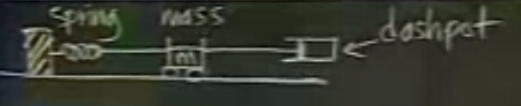
\includegraphics[height=2cm]{9_1.png}

Eksen yatay oldugu icin ona $x$ degiskenini atayalim, tabii bu yuzden
ODE'deki bagimli degisken o olacak, yani ustteki $y$ yerine $x$
kullaniyoruz. Kafa karistirmasin diye vurguladik, cunku cogunlukla $x$ bagimsiz
degisken olarak kullanilir. 

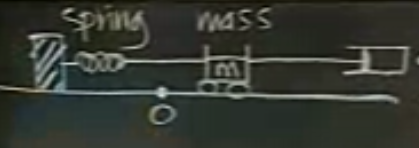
\includegraphics[height=2cm]{9_2.png}

Devam edelim. Diyelim ki 0 ile isaretlenen yer bir denge noktasi. Yani bu
noktada hem yayin, hem de engelleyicinin itme / cekme noktasi tatmin
ediliyor durumda. Eger o noktadan daha sola gidersek, yay itmeye ugrasacak,
saga gidersek cekmeye ugrasacak, tabii engelleyici de birseyler yapacak. 

Denklem soyle: 

\[ \underbrace{mx''}_{Kuvvet} =
- \underbrace{kx}_{Yay} 
- \underbrace{cx'}_{Engelleniyici}
\]

$mx''$ sistemde ortadaki kutlenin uyguladigi kuvvettir, arti, eksi olmasi
kuvvetin sag ya da sol yonunde oldugunu gosterir. Bu kuvvet Newton Kanunu'na
gore ivme (ikinci turev, $x''$) ve kutlenin carpimidir. Unutmayalim,
bagimsiz degisken $t$, o zaman $x'$ hiz, $x''$ ivme.

Sistemdeki yay sadece kutleye ``tepki'' verir, kutle ne yapiyorsa tersini
yapar. Eger kutle sola gelirse saga, saga gelirse sola dogru karsi kuvvet
uygular, o yuzden ve esitligin saginda oldugu icin sistemde $-kx$ (ters
isaret) ile belirtildi (eksiyi tekrar artiya cevirmek icin). Bu tepkinin
alinan mesafe $x$ ile orantili (bir sabitle carpilarak) olmasi Hooke
Kanunu'ndan ileri geliyor.

Engelleyici ise yaya benziyor ama onun tepkisi hiz ile orantili, mesafe ile
degil. Bu mekanizmaya sahip olan kapilari hatirlayin, cok hizli kapatmaya
ugrasinca cok daha sert engelleme yaparlar. Bu tepki, yine ters isaretle
$-cx'$ ama birinci tureve (hiz) icerecek sekilde temsil edilir.

Nihai denklem ise soyle

\[ mx'' + cx' + kx = 0 \]

\[ x'' + \frac{c}{m}x' + \frac{k}{m}x = 0 \]

ODE'yi cozmek icin 2 cozum bulmak gerekir. 

2 cozumun birbirinden bagimsiz olmasi lazimdir, yani mesela $y_1$
bulunmussa, $y_2$ onun bir sabitle carpilmis hali olamaz. Cunku sabitlerle
carpma isi denklemde zaten rasgele sabitlerin isi, iki cozum birbirinin
kati ise o zaman genel cozumu yaratamayiz, cunku rasgele sabitlerin isi
zaten yapilmis olur.

Cozum icin en basit, temel yontem tahmin etmektir. $y = e^{rt}$ cozumunu
deneyelim deriz. Niye $e^{rt}$? Turevini, entegralini almak kolay. Yerine
koyalim. 

\[ r^2e^{rt} + Are^{rt} + Be^{rt} = 0 \]

Oyle bir $r$ bulalim ki denklemin sol tarafi sifir olsun. $e^{rt}$ hicbir
zaman sifir olamayacagina gore sifirlik denklemin ``geri kalaninda''
demektir, $e^{rt}$'yi iptal edelim. 

\[ r^2 + Ar + B = 0 \]

Bu bir karesel denklemdir! Cozumu lisede ogretilir. Bu denkleme ODE'nin
(ya da yay / kutle sisteminin) karakteristik denklemi ismi de verilir.

1. Durum: kokler reel ve $r_1 \ne r_2$

Bu en basit, direk sonuc. O zaman nihai cozum

\[ y = c_1 e^{r_1t} + c_2  e^{r_2t}\]

Ornek

\[ y'' + 4y' + 3y = 0 \]

Karakteristik denklem

\[ r^2 + 4r + 3 = 0 \]

\[ (r+3)(r+1) = 0 \]

Genel cozum

\[ y = c_1e^{-3t} + c_2e^{-t} \]

Baslangic sartlari 

\[ y(0) = 1 \]

\[ y'(0) = 0 \]

Sartlar ne anlama geliyor? $t=0$'da, baslangicta, kutle $x=1$
noktasinda. Yani yay saga dogru gerilmis olacak. Ikinci sart sisteme
baslangicta disaridan ek bir guc vermiyoruz demek, $x=1$ noktasina
getiriyoruz, ve birakiyoruz. Birakinca kutlenin sola, sonra saga, vs. gidip
gelecegini tahmin edebiliriz. 

Iki kosul var, cunku bulmamiz gereken iki sabit var. 

Kosullarin ikincisi icin tureve ihtiyac var, turevi hesaplayalim

\[ y' = -3c_1e^{-3t} + - c_2 e^{-t} \]

$t = 0$ ise, $y$ formulu (ilk kosul) $1 = c_1 + c_2$ olur. Ikinci kosul
$0 =
-3c_1 - c_2$. 

Simdi elimizde beraber cozulecek (simultaneous) iki tane lineer denklem
var. Bunlari cozmeyi de lisede ogrenmistik. Bu arada karesel denklemler, ve
ustteki tur lineer denklemlerin cozumunun en onemli uygulama alani
isledigimiz turden fiziksel problemler icindir. Lise cagi bizi bunlar icin
hazirliyormus demek ki.

\[ c_1 = -1/2 \]

\[ c_2 = 3/2 \]

Cozum: 

\[ y = -\frac{1}{2}e^{-3t} + \frac{3}{2}e^{-t} \]

Peki bu cozum grafiksel olarak neye benzer? Iki ustel fonksiyonun
kombinasyonunu elle cizmek pek kolay degildir, onun icin bilgisayari
kullanmak daha iyi. 

2. Durum: kokler kompleks 

$r = a \pm bi$

Bu sekilde bir $r$ cozume nasil etki eder? Cozum

\[ y = e^{(a+bi)t} \] 

seklinde olacaktir, fakat bu cozumun bizim icin hicbir anlami yok. Biz
$y$'nin, $x$'in nasil davrandigini gormek istiyoruz. Su teori yardimimiza
yetisiyor: 

Teori: Eger $u + iv$ kompleks sayisi, $y'' + Ay' + By = 0$ reel ODE
denkleminin kompleks cozumu ise o zaman $u$ ve $v$ reel cozum icin
kullanilabilirler.

Ispat: Cozum olmak ne demek? Su denklemin dogru olmasi demek: 

\[ (u+iv)'' + A(u+iv)' + B(u+iv) = 0\]

Reel ve hayali kisimlarina ayiralim

\[ 
\underbrace{u'' + Au' + Bu}_{reel} + 
i\underbrace{(v'' + Av' + Bv)}_{hayali} = 0
\]

Ustteki denklemin sol tarafinin sifira esit olmasinin tek yolu, hem reel,
hem hayali bolumun sifira esit olmasidir. Onlarin sifira esit olmasi demek
her iki denklemin de ana denklem olan $y'' + Ay' + By = 0$'a tipatip
benzemeleri demektir. O zaman hem $u$, hem $v$ ana ODE icin bir cozumdur. 

Bu arada ispatta $A$ ve $B$'nin reel olmasi zorunlulugunu dolayli olarak
kullandik, cunku eger $A$ ve $B$ hayali olabilseydi, ustteki denklemdeki
reel bolume reel diyemezdik, denklemin tamamini ustteki sekilde
gruplayamazdik, ve hayali bir sayinin sifira esitlenebilmesi icin
yuruttugumuz mantigi yurutemezdik. O zaman neresi reel neresi hayali
olacakti? 

Cozume donelim. 

\[ y = e^{(a+bi)t} \] 

Ustel kompleks degerler ve cos, sin formuna gecisi hatirlayalim

\[ e^{i\theta} = \cos \theta + i\sin \theta \]

O zaman usttekini genisleterek devam edelim

\[ y = e^{at} e^{ibt} \]

Sadece ikinci kisim cos, sin formuna cevirilebilir

\[ e^{ibt} = cos(bt) + isin(bt) \]

Biraraya koyarsak

\[ y = e^{at} (cos(bt) + isin(bt)) \]

Reel bolum

\[ y = e^{at}cos(bt) \] 

Hayali bolum

\[ y = e^{at}sin(bt) \] 

O zaman cozum

\[ y = e^{at} \bigg( c_1 \ cos(bt) + c_2 \ sin(bt) \bigg) \]

Bu fonksiyon neye benzer? Dikkat edelim, $e^{at}$ yuksekligi (amplitude)
kontrol ediyor, geri kalani iki sinusoidal salinimin kombinasyonu, farkli
yukseligi ama ayni frekansi olan iki salinim. Bu yuzden onlarin toplami da
bir sinusoidal salinim. Bu fonksiyon aslinda daha onceki bir derste
bahsedilen bir trigonometrik esitligi kullanmak icin de uygun [hoca
herhalde 8. dersteki esitlikten bahsediyor].

Simdi engelleyici / amortisor (damping) faktorunu degistirelim. Onceki
ornekte amortisor zayifti, yayin etkisi daha fazlaydi, zaten o sebeple bir
salinim gormustuk, bu kutleyi birakinca bir sure saga, sola sallanmasi
demekti. Yeni denklem:

\[ y'' + 4y' + 5 \]

Karakteristik denklem

\[ r^2 + 4r + 5 = 0 \]

\[ r = -4 \pm \frac{\sqrt{-4}}{2} = -2 \pm i\]

Cozum

\[ e^{(-2+i)t} \]

Reel cozum

\[ e^{-2t}\cos t \ , \ e^{-2t}\sin t\]

\[ y = e^{-2t} (c_1 \cos t + c_2 \sin t) \]

Baslangic sartlari yine ayni olsun

\[ y(0) = 1 \]

\[ y'(0) = 0 \]

Hesabi yaptiktan sonra sonuc

\[ y = e^{-2t} (\cos t + 2 \sin t) \]

Trigonometrik esitligi kullanalim

\[ = \sqrt{5}e^{-2t} cos (t - \phi) \]

$\sqrt{5}$ nasil bulundu? Onceki dersten su ucgeni hatirlayalim

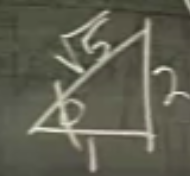
\includegraphics[height=2cm]{9_3.png}

O zaman $\phi \approx 70^{o} \pm 5$

Cozumun grafigini cizersek

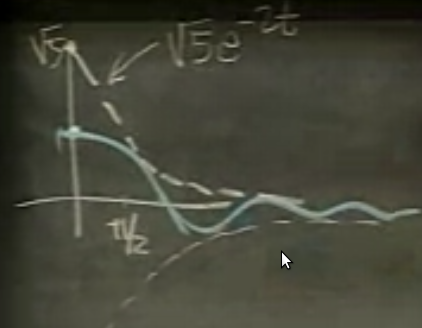
\includegraphics[height=4cm]{9_4.png}

Bu yetersiz amortisorlu (underdamped) durumudur. 

Simdi amortisorun ne az, ne de fazla oldugu duruma bakalim. Burada
amortisor ``tam yerinde'', bu kosula kritik amortisorlu sart (critically
damped) deniyor. Karakteristik denklemdeki kokler ayri ve reel degil,
kompleks degil. Reel ama birbirine esit, diyelim ki $r = -a$. 

\[ (r+a)^2 = 0 \]

\[ r^2 + 2ar + a^2 = 0 \]

ODE

\[ y'' + 2ay' + a^2y = 0 \]

Yani yay sabiti ve amortisor sabiti arasinda bir iliski var. 

Fakat burada bir problem var. Cozumlerden biri $e^{-at}$ evet, ama bu
elimdeki tek cozum. 2. derece ODE icin iki cozum lazim. 

Gerekli ikinci cozumu elde etmenin degisik yollari var. Bir tanesi soyle:

Eger $y'' + py' + qy = 0$ icin bir $y_1$ cozumu biliyorsak, $y = y_1 u$
seklinde ikinci bir cozum de muhakkak vardir. $u$'yu nasil
hesaplayabilecegimizi gorelim.

Elimizde $y = e^{-at}$ var. $y'' + 2ay' + a^2y = 0$ icin bir $u$ bulacagiz,
yani su formda bir cozum arayacagiz

\[ y = e^{-at} u \]

Birinci turev

\[ y' = -a e^{-at}u + e^{-at} u' \]

Bunun bir kere daha turevini alalim

\[ a^2e^{-at}u - 2ae^{-at}u' + e^{-at}u'' \]

Ustteki uc denklemden en alttakini 1 ile carpariz (yani degismez),
ortadakini $2a$ ile caprariz, bastakini $a^2$ ile carpariz. Bu carpimlari
toplariz, esitligin sol tarafinda 0 elde ederiz. Esitligin sag tarafindaki
neredeyse her terim toplanarak sifir hale gelir, sadece $e^{-at}u''$ geriye
kalir. O zaman sunu soyleyebiliriz:

\[ e^{-at} = 0 \]

Demek ki 

\[ u'' = 0 \]

Bu ne demektir?

\[ u = c_1t + c_2 \]

Oyle degil mi? Ikinci turevi sifir olan sey nedir? Ustteki form'daki bir
formuldur, $c_1$ ve $c_2$ rasgele iki sabittir. Birinci turevi alirken $c_2$
yokolacakti $c_1$ kalacakti, ikinciyi alirken $c_1$ yokolacakti. 

Bu sonuc bana bir suru cozum bulma imkani saglar, ama sadece tek basina
$t$'yi bile kullansam olur, cunku bana $e^{-at}$'den farkli sadece bir tane
daha cozum lazim. O zaman ikinci cozum su olabilir:

\[ y_2 = e^{-at} \cdot t \]

Kritik amortisor durumunun cozumu de budur. 

* * * 

Ekler

Teori

Eger $y=f_1(x)$ ve $y=f_2(x)$ su diferansiyel denklemin cozumu ise

\[ \frac{d^ny}{dx^n} + a_1 \frac{d^{n-1}y}{dx^{n-1}} + .. + a_n y = 0\]


O zaman $y=c_1f_1(x) + c_2f_2(x)$ te ayni diferansiyel denklemin bir
cozumudur, ki $c_1$ ve $c_2$ herhangi bir (arbitrary) sabit degerler olabilirler.

Ispat

Eger $f_1$ bir cozum ise, diferansiyel denklemde $y$ yerine koyabilmemiz
gerekir, $f_2$ ve $c_1f_1 + c_2f_2$, ayni sekilde. Hepsine bakalim.

\[ \frac{d^nf_1}{dx^n} + a_1 \frac{d^{n-1}f_1}{dx^{n-1}} + .. + a_n f_1 = 0\]

\[ \frac{d^nf_2}{dx^n} + a_1 \frac{d^{n-1}f_2}{dx^{n-1}} + .. + a_n f_2 = 0\]

\[ \frac{d^n(c_1f_1 + c_2f_2)}{dx^n} + 
a_1 \frac{d^{n-1}(c_1f_1 + c_2f_2)}{dx^{n-1}} + .. + 
a_n (c_1f_1 + c_2f_2) = 0
\]

Sonuncu formul icin $c_1$ ve $c_2$'leri disari cekip gruplamayi onlara gore
yaparsak

\[ 
c_1 \bigg[
\frac{d^nf_1}{dx^n} + a_1 \frac{d^{n-1}f_1}{dx^{n-1}} + .. + a_n f_1
\bigg] +
c_2 \bigg[
\frac{d^nf_2}{dx^n} + a_1 \frac{d^{n-1}f_2}{dx^{n-1}} + .. + a_n f_2
\bigg]
 \]

Buyuk parantezler icindeki degerler diferansiyel denklemin $f_1$ ve $f_2$
kullanilarak acilmis hali degil mi? O zaman o degerler sifir. Yani

\[ c_1 \cdot 0 + c_2 \cdot 0 \]

Bu deger de tabii ki sifira esit. 

\[ c_1 \cdot 0 + c_2 \cdot 0 = 0\]

ve bu sifir sonucu, ana diferansiyel denklemin sonucuyla ayni. O zaman
ispat tamamlanmis demektir.

Kaynaklar 

Differential Equations, Hari Kishnan, sf. 118

\end{document}











